\chapter{Fundamentação Teórica}
\label{chap:fund}

Neste capítulo serão abordados os principais conceitos de \emph{Deep Learning}, assim como as técnicas e algoritmos aplicados para auxiliar os profissionais de laboratório a realizarem exames de sangue de uma forma automatizada e eficiente. Além disso, será detalhado sobre os hemogramas e diferentes dados coletados através de uma análise de sangue.

\section{Exames Laboratoriais de Sangue}
\label{sec:conceito1}
Os exames laboratoriais de sangue, principalmente se tratando de hemogramas, são um tipo de exame simples porém de extrema importância para a saúde humana. Através desses exames se pode descobrir diversas informações sobre o organismo da pessoa em questão, inclusive detectar doenças e problemas de forma antecipada, como por exemplo para diagnosticar anemia, deficiências nutricionais, parasitas no sangue, doenças virais e autoimunes. Também é possível se identificar infecções, doenças como leucemia, diagnosticar efeitos de medicamentos e também o efeito de vários tipos de estresse sobre o corpo \cite{abcOfCbc, atlasDeHematologiaEAnalise}.

Um exame poderá ser solicitado por um médico, ou a partir do interesse do próprio paciente, e realizado em um laboratório de confiança, que será responsável por realizar a coleta, encaminhar para a análise específica e retornar o resultado. Todo esse processo é custoso em tempo de espera e também financeiramente, pois o maquinário para esse tipo de atividade é muito caro para aquisição e manutenção.

\subsection{Sangue}
O sangue é um elemento do corpo humano, que circula em estado líquido através de todo o sistema circulatório do organismo, sendo de importância para o funcionamento correto das células através da entrada e saída de substâncias que podem modificar a sua composição \cite{manualHematologia}.

Pode ser dividido em duas principais partes, sendo o plasma ou soro, a parte de transporte das substâncias pelo sistema, formado pela ingestão de água e alimentos, essas duas nomenclaturas existem de acordo com o uso ou não de anticoagulantes para a separação do sangue, onde dependendo do objetivo e foco da análise, se pode adotar uma ou outra \cite{manualHematologia}.

A segunda parte do sangue, que será objeto de estudo para este trabalho, é a parte celular que contém todas as células presentes no sangue e se classificam como glóbulos vermelhos, glóbulos brancos e plaquetas. Geralmente observa-se a presença de eritrócitos, vários tipos e classes de leucócitos e as plaquetas como um todo, que serão abordados um a um posteriormente \cite{manualHematologia}.

\subsubsection{Glóbulos Vermelhos}
Os glóbulos vermelhos, também conhecidos como \emph{Red Blood Cells (RBC)}, são as hemácias presentes no sangue, também podem ser citadas em exames e registros médicos como eritrócitos, essas células são pequenas e circulares, geralmente em formatos de discos e não possuem núcleo. Estão presentes em grande quantidade, possuindo uma vida útil de aproximadamente 120 dias até que o próprio sistema as elimine \cite{manualHematologia}.

É indispensável ao falar sobre a parte vermelha do sangue, citar a hemoglobina que é uma proteína presente nas hemácias e de extrema importância para o funcionamento do sistema, pois através dela é possível realizar o transporte de oxigênio e gás carbônico pelo sistema sanguíneo, permitindo as trocas gasosas necessárias \cite{manualHematologia}.

\begin{figure}[!htb]
	\centering
	\caption{Glóbulos Vermelhos (RBC)}
	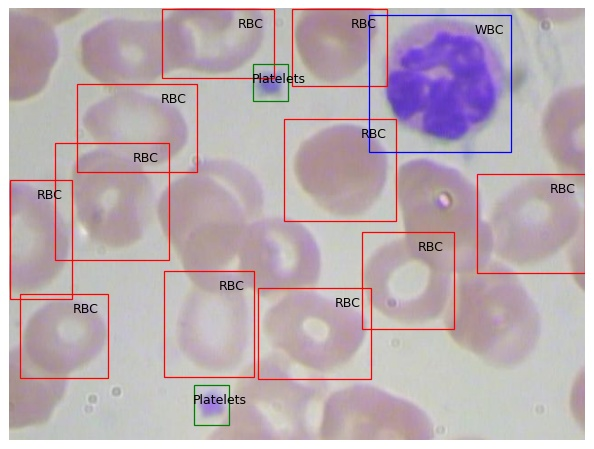
\includegraphics[width=0.40\textwidth]{img/rbc.jpg}
	\legend{Fonte: \cite{datasetBCCD}}
	\label{fig:rbc}
\end{figure}
 
\subsubsection{Glóbulos Brancos}
Os glóbulos brancos, também conhecidos como \emph{White Blood Cells (WBC)}, são as células brancas do sangue, sendo responsáveis pela defesa do organismo contra as principais ameaças do corpo humano presentes no sistema sanguíneo. Através da fagocitose, que é um processo de englobamento de partículas sólidas pelas células, é realizado ações de defesa contra a invasão de fragmentos estranhos. Os glóbulos brancos são criados na medula óssea e estão presentes em todo o sangue, também em grande quantidade \cite{manualHematologia}.

Se faz necessário a classificação dos diferentes tipos de células brancas e de suas importâncias para o sistema de defesa do organismo. É importante frisar que essa classificação se refere aos leucócitos maduros, mas também se pode encontrar presente os leucócitos imaturos (promielócitos, mielócitos, metamielócitos) \cite{manualHematologia}.

\begin{figure}[!htb]
	\centering
	\caption{Glóbulos Brancos (WBC)}
	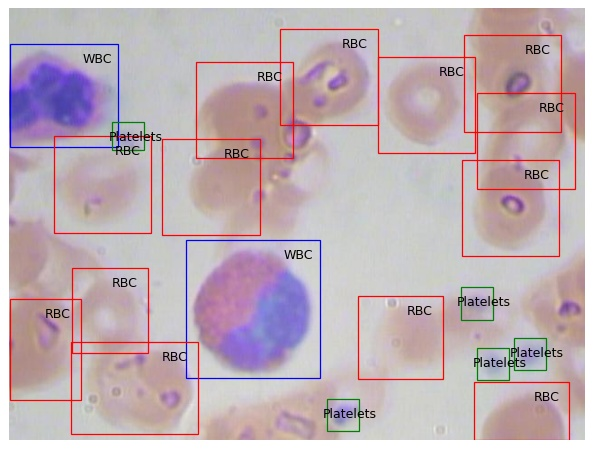
\includegraphics[width=0.40\textwidth]{img/wbc.jpg}
	\legend{Fonte: \cite{datasetBCCD}}
	\label{fig:wbc}
\end{figure}
 
\begin{itemize}
	\item \textbf{Neutrófilos}: células brancas mais abundantes capazes de entrar nos tecidos, onde conseguem realizar a defesa do organismo, fagocitando partículas estranhas. Essas células são conhecidas como neutrófilos segmentados, pois existe uma célula percursora, que é o bastão, ou também chamado de neutrófilos bastonetes, que possuem essa nomenclatura pois seu núcleo não está amadurecido, ou seja ainda são jovens, e geralmente são identificados quando há infecções em fase aguda. 
	\item \textbf{Eosinófilos}: células brancas responsáveis na defesa contra parasitas, geralmente estão presentes em grande quantidade no sangue durante reações alérgicas e infestações parasitárias.
	\item \textbf{Basófilos}: células brancas atuantes em respostas alérgicas e na coagulação do sangue. São capazes de liberar histamina, contribuindo para respostas alérgicas ao dilatar e permeabilizar os vasos sanguíneos e também liberam heparina que é capaz de prevenir a coagulação do sangue.
	\item \textbf{Monócitos}: células brancas capazes de entrar no tecido conjuntivo frouxo, onde conseguem se desenvolver em grandes células com grande efeito fagocítico denominadas macrófagos, de forma a ingerir partículas estranhas ao organismo.
	\item \textbf{Linfócitos}: segundo tipo de célula branca mais abundante, são responsáveis e de extrema importância nas respostas imunes específicas do corpo humano, inclusive na produção de anticorpos.
\end{itemize}

\subsubsection{Plaquetas}
As plaquetas, também conhecidas e citadas como \emph{Platelets}, são os menores componentes do sangue e possuem grande responsabilidade na hemostasia, que é uma resposta fisiológica para a prevenção e interrupção de sangramentos e hemorragias, ou seja, elas atuam na manutenção dos vasos sanguíneos. As plaquetas são fragmentos do citoplasma de megacariócitos, ou seja, elas são produzidas na medula óssea como parte dessas células especializadas que irão se dividir posteriormente e gerar um grande número de plaquetas. Aproximadamente, para cada 1 megacariócito, se pode produzir cerca de 4000 plaquetas \cite{abcOfCbc}.

Devido ao fato de serem fragmentos de uma célula, as plaquetas não possuem núcleo e são muito pequenas, com aproximadamente de 1–3 µm de diâmetro, com a coloração azul-acinzentado. A vida útil das plaquetas dura em média de 9 a 12 dias, e elas são removidas pelo baço quando estão velhas ou danificadas \cite{abcOfCbc}.

\begin{figure}[!htb]
	\centering
	\caption{Plaquetas (Platelets)}
	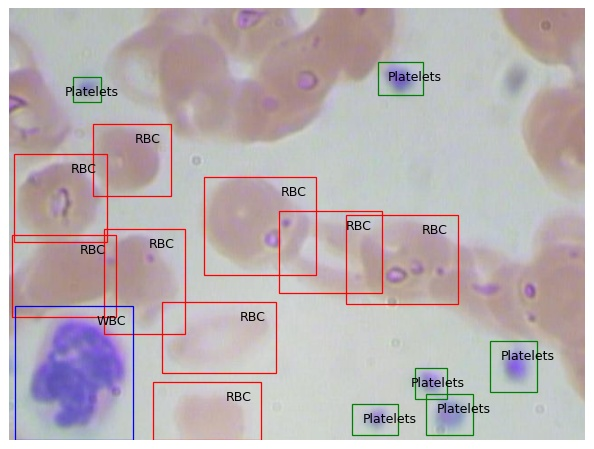
\includegraphics[width=0.40\textwidth]{img/plt.jpg}
	\legend{Fonte: \cite{datasetBCCD}}
	\label{fig:plaquetas}
\end{figure}
 
\subsection{Hemograma}
Um hemograma, também conhecido e citado como \emph{Complete Blood Count (CBC)}, é um exame bastante comum e muito utilizado, onde se realiza uma análise de sangue que envolve a contagem das diferentes células sanguíneas. A partir dos números obtidos através dessa contagem e com a comparação desse valor com as faixas de normalidade, é possível chegar a diversas conclusões sobre a saúde do paciente e até mesmo já identificar alguma doença ou problema \cite{manualHematologia, abcOfCbc}.

Um hemograma geralmente é realizado em duas principais etapas, sendo a primeira relacionada ao eritrograma que se refere à análise das células vermelhas, de forma a revelar até mesmo alguns tipos essenciais de alterações patológicas do sistema eritropoético, que é o sistema responsável pela produção do material vermelho do sangue, como aumento na produção de glóbulos vermelhos e anemias. A segunda parte está relacionada com o leucograma, que corresponde à contagem global e específica dos leucócitos, a parte branca do sangue. O quadro leucocitário resultante com o exame hematológico, possibilita ao médico tirar importantes conclusões \cite{manualHematologia, abcOfCbc}.

\subsubsection{Eritrograma}
O objetivo do eritrograma ao realizar a análise da parte vermelha do sangue, é analisar alguns atributos chave, primeiramente é realizado a contagem geral dos eritrócitos adotando uma escala de milhões/mm³. A hemoglobina também será calculada e registrada em uma escala de g/dl \cite{interpretacaoHemograma, manualHematologia}.

Depois dessa principal contagem é calculado alguns índices importantes, sendo o primeiro deles o cálculo do volume corpuscular médio (VCM), que é o volume médio das hemácias, calculado pelo quociente de um determinado volume de hemácias pelo número de células contidas no mesmo volume. Outro importante atributo é a hemoglobina corpuscular média (HCM), que semelhante ao VCM, é o conteúdo médio da hemoglobina, calculado pelo quociente de conteúdo de hemoglobina em um determinado volume de hemácias pelo número de células contidas no mesmo volume \cite{interpretacaoHemograma, manualHematologia}.

Também temos outro índice que é a concentração de hemoglobina corpuscular média (CHCM), sendo a percentagem da hemoglobina em uma amostra de 100ml de hemácias. Por fim temos, a amplitude de distribuição dos glóbulos vermelhos, que em inglês significa \emph{Red Cell Distribution Width (RDW)}, que será responsável por avaliar a variação de tamanho entre as hemácias \cite{interpretacaoHemograma, manualHematologia}.

\begin{figure}[!htb]
	\centering
	\caption{Exemplo de Eritrograma e seus Atributos}
	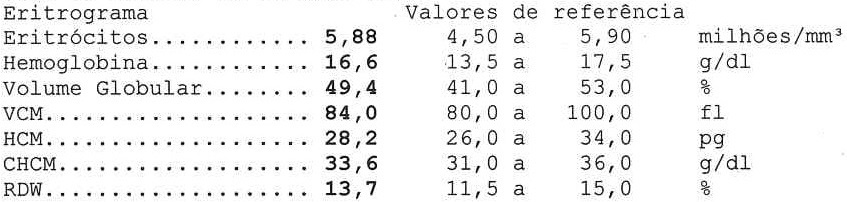
\includegraphics[width=0.80\textwidth]{img/eritrograma.jpg}
	\legend{Fonte: Elaborada pelo autor.}
	\label{fig:eritrograma}
\end{figure}
 
\subsubsection{Leucograma}
O objetivo do leucograma ao realizar a análise da parte branca do sangue, assim como no eritrograma, é analisar alguns atributos chave, porém diferente do processo anterior, essa etapa terá um foco muito maior na classificação e contagem de diferentes células brancas.

Primeiramente é feita uma contagem geral de leucócitos em mm³. Depois é realizada a contagem de forma a classificar cada tipo de leucócito presente, com neutrófilos, eosinófilos, basófilos, linfócitos, monócitos e também os granulócitos imaturos (promielócitos, mielócitos, metamielócitos). Por fim, também é calculado o número presente de plaquetas no sangue em mm³ \cite{interpretacaoHemograma, manualHematologia}.

\begin{figure}[!htb]
	\centering
	\caption{Exemplo de Leucograma e seus Atributos}
	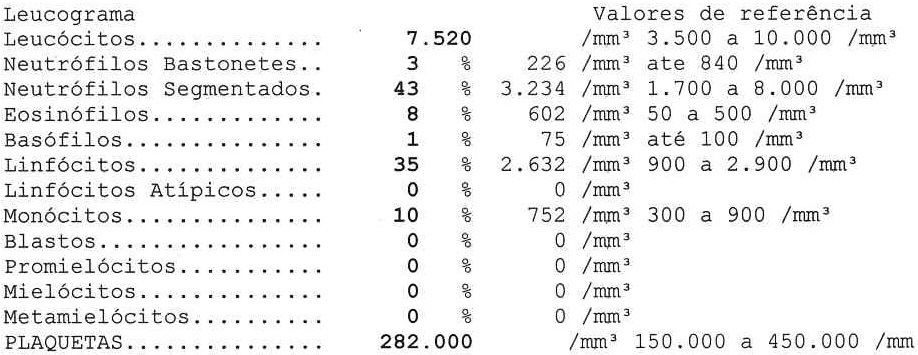
\includegraphics[width=0.80\textwidth]{img/leucograma.jpg}
	\legend{Fonte: Elaborada pelo autor.}
	\label{fig:leucograma}
\end{figure}

\section{Inteligência Artificial: Machine Learning e Deep Learning}
\label{sec:conceito2}
A abordagem de Deep Learning que é objeto de estudo desse trabalho é uma das subareas de Machine Learning que por sua vez é subarea de Inteligência Artificial, portanto antes de abordar cada um desses conceitos, quais suas diferenças e aplicações, se faz necessário explicar e citar sobre a Inteligência Artificial.

A Inteligência Artificial é uma abordagem para a resolução de problemas de diversas naturezas através de uma forma automatizada, ou seja, é uma maneira de se resolver problemas sem a necessidade de um humano ou usuário específico para esse trabalho. Essa área está muito em alta nos dias de hoje, buscando cada vez novas maneiras de automatizar a vida humana. Podemos encontrar essa abordagem em diversos segmentos da indústria e atualmente também vem crescendo o uso dentro das residências para os mais diversos usos.

O intuito dessa área é buscar formas de ensinar máquinas e computadores a serem capazes de ter uma inteligência cada vez mais semelhante aos seres humanos, isso ocorre geralmente através do reconhecimento de padrões por esses dispositivos, onde eles serão ensinados a analisar dados e interpretar de alguma forma, muito semelhante ao que acontece para o aprendizado de seres humanos. Porém, diferente de nós, as máquinas geralmente precisam de um volume massivo de dados para que sejam capazes de aprender algo básico.

\subsection{Machine Learning}
A resolução de problemas através de ferramentas da computação é bastante comum e para isso se faz uso de algortmos programados para essa finalidade específica, porém não é em todos os problemas que podemos aplicar essa abordagem tradicional, devido ao fato de que nem sempre se sabe um caminho único de etapas a serem seguidas para resolução dos problemas. No caso, quando se sabe a entrada de dados e o resultado onde queremos chegar, mas não os meios para se chegar nesse resultado, se deve utilizar um modelo de Machine Learning para realizar a predição. Podemos pensar que na abordagem de algoritmos tradicionais de programação possuímos os parametros necessários e conhecemos o método para assim chegar ao resultado, mas na aplicação de machine learning, conhecemos os parametros e o resultado, porém o método será aprendido e apresentado pela máquina. %Citar o livro 1

Podemos pensar em um modelo de Machine Learning como uma criança que está a aprender algo novo, logo todo modelo passará por três principais etapas, primeiramente o pré-processamento dos dados, depois pela fase de treinamento e por fim será realizado os devidos testes. Dessa forma, um modelo de Machine Learning deverá ser treinado antes de realizar a predição de qualquer valor ou resultado, onde o responsável pelo treinamento deverá fornecer um grande volume de dados, assim como os resultados esperados por cada um deles. Dessa forma o modelo poderá aprender a entender e interpretar os dados de forma correta, para assim ser capaz de reproduzir esse mecanismo para prever o resultado de futuros dados.

Após o treinamento do modelo como um todo, na fase de teste, para testar e avaliar o treinamento do modelo, também é possível aplicar algumas formas e técnicas para medir o desempenho como um todo, apontando fatores interessantes como o nível de assertividade, a precisão e também o número de acertos e erros relacionados com falsos positivos e falsos negativos através de uma matriz de confusão.

%Imagem da Matriz de Confusão

Existem várias abordagens de Machine Learning e elas podem ser classificadas em várias categorias diferentes, porém sempre podemos dividir em duas principais abordagens mais utilizadas, sendo elas a regressão e a classificação. Os modelos de regressão serão responsáveis pela predição de valores reais, enquanto que os modelos de classificação serão responsáveis pela rotulação dos dados em determinadas classes. Além disso, também podemos classficar os algoritmos em supervisionados ou não supervisionados. No aprendizado supervisionado, sabemos o resultado correto, ou seja, onde o modelo deverá chegar a partir dos dados obtidos, porém no aprendizado não supervisionado, o modelo terá que lidar com dados não estruturados e sem um resultado claro. %Citar livro 2

\subsection{Deep Learning}
Existe alguns casos que o Machine Learning não é suficiente para o aprendizado a partir dos dados, isso ocorre pois o aprendizado acontece através de reconhecimento de padrões com base nos dados e esses dados não podem ser utilizados de qualquer forma, devem ser preparados e adaptados para cada modelo, ou seja, a máquina não será capaz de aprender por conta própria pois sempre precisará de intervensão humana para o processamento dos dados. Logo se necessita de uma abordagem muito mais parecida com a forma de pensar dos seres humanos, como o Deep Learning. %Citar livro penultimo

O Deep Learning busca uma abordagem bastante parecida com o cérebro humano, isso acontece pois utiliza uma estrutura composta de perceptrons, que são uma versão computadorizada de algo parecido com um neurônio humano. O perceptron será capaz de receber inputs, ou seja dados de entrada, e reproduzir uma saída esperada, bastante parecido com os modelos de machine learning como visto anteriormente, porém a diferança desse método é a sua utilização, pois não se usará apenas um perceptron, para se assemelhar ao cérebro humano serão utilizados diversos perceptrons, em diferentes camadas dentro do modelo, podemos chamar toda essa estrutura de rede neural artificial ou artificial neural network (ANN). %Conferir e complementar sobre o Perceptron %Falar de Neural Network %Citar ultimo Livro

As camadas utilizadas no Deep Learning, podem conter um número variável de perceptrons. Onde geralmente se adotará uma camada de entrada para os inputs e uma camada de saída para os outputs, que são justamente o resultado esperado ou proposto. Entre essas camadas terá as camadas ocultas, que serão responsáveis por toda a parte lógica do sistema. %Falar mais sobre as camadas

Como a ANN Aprende?
A ANN aprende com base no uso de um algoritmo de backpropagation, que significa propagação regressiva, durante o treinamento ocorre o uso desse recurso, onde primeiramente ele irá inicialiar a rede com pesos aleatórios,

2. For all training cases, follow these steps:
° Forward pass: Calculates the network's error, that is, the difference 
between the desired output and the actual output
° Backward pass: For all layers, starting with the output layer back to 
input layer:
i: Shows the network layer's output with the correct input (error 
function).
ii: Adapts the weights in the current layer to minimize the error 
function. This is backpropagation's optimization step.

O processo de treinamento irá terminar quando o erro no dataset de validação começar aumentar, isso ocorre pois nesse momento ocorre o inicio de uma fase de overfitting, onde basicamente o algoritmo não será capaz de interpretar novos dados a não ser aqueles que ele foi treinado.

The training process ends when the error on the validation set begins to increase 
because this could mark the beginning of a phase overfitting, that is, the phase 
in which the network tends to interpolate the training data at the expense of 
generalizability.

Otimização dos pesos
A Otimização de pesos é um componente essencial para uma rede neural funcionar, para isso são escolhidos valores aleátorios como parâmetros iniciais para o modelo, é computado



Weight optimization
The availability of efficient algorithms to optimize weights, therefore, constitutes an 
essential tool for the construction of neural networks. The problem can be solved 
with an iterative numerical technique called Gradient Descent (GD). This technique
works according to the following algorithm:
1. Randomly choose initial values for the parameters of the model
2. Compute the gradient G of the error function with respect to each parameter 
of the model
3. Change the model's parameters so that they move in the direction of 
decreasing the error, that is, in the direction of -G
4. Repeat steps 2 and 3 until the value of G approaches zero
The gradient (G) of the error function E provides the direction in which the error 
function with the current values has the steeper slope; so to decrease E, we have to 
make some small steps in the opposite direction, -G.
By repeating this operation several times in an iterative manner, we move down
towards the minimum of E, to reach a point where G = 0, in such a way that no 
further progress is possible:


%Possivel Imagem de ajuste de pesos

The learning process of a neural network is configured as an iterative process of the 
optimization of the weights and is therefore of the supervised type. The weights are 
modified because of the network's performance on a set of examples belonging to the 
training set, that is, the set where you know the classes that the examples belong to. 
The aim is to minimize the loss function, which indicates the degree to which the 
behavior of the network deviates from the desired behavior. The performance of the 
network is then verified on a testing set consisting of objects (for example, images in 
an image classification problem) other than those in the training set.

\subsubsection{Métodos}
DNN E depois CNN e RNN
Convolutional Neural Network (CNN)
%Diferentes tipos de organizações de camadas
%Imagens

\subsubsection{Bibliotecas e Recursos}
%TensorFlow e Keras
%Exemplo do TensorFlow de imagens
%Citar livro 3

%Todos os livros que eu peguei tem boas referências

\chapter{Estado da Arte da Área Pesquisada}
\label{chap:mapeamento}

O processo de pesquisa e seleção dos trabalhos relacionados, foi realizado com base em um mapeamento sistemático sobre as pesquisas com propostas para agilizar a identificação e interpretação de análises de sangue. Esta revisão resultou na identificação e seleção dos principais trabalhos de pesquisa no tema deste Projeto de Trabalho de Conclusão de Curso. Outro objetivo deste mapeamento sistemático foi verificar os métodos utilizados para a aplicação de Deep Learning em imagens de sangue em placas de petri de maneira que possam ser aplicados neste projeto de forma satisfatória.

\section{Mapeamento Sistemático da Literatura}

O mapeamento sistemático da literatura é realizado com base na busca e levantamento de artigos, para isso se utiliza uma string de busca para as principais bibliotecas e repositórios de artigos. Esses artigos serão analisados e selecionados conforme a sua área de pesquisa e a sua temática, para inclusão nesse estudo. Para isso, se é utilizado uma ferramenta para automatização dessa tarefa, que é o Parsifal\footnote[1]{https://parsif.al/}, de modo a definir a string de busca, salvar os artigos necessários e realizar a seleção.

As questões de pesquisas levantadas para isso foram, ``Como os algoritmos de Deep Learning podem ser utilizados para a interpretação de exames?'' e ``Como realizar o tratamento de imagens para reconhecimento por modelos de Deep Learning?''. A partir dessas questões se foram extraídas palavras e termos para o direcionamento da pesquisa. Podemos visualizar estas palavras com seus sinônimos na Tabela 1.

\begin{table}[!htb]
	\centering
	\caption{Palavras-Chave e Sinônimos}
	\label{tbl:palavrasChave}
	\begin{tabular}{|c|c|}
		\hline
		\textbf{Palavra-Chave} & \textbf{Sinônimos}                                        \\ \hline
		Blood Analysis         & Blood Sample                                               \\ \hline
		Classification         & Interpretation, Recognition                                \\ \hline
		Deep Learning          & Artificial Intelligence, Computer Vision, Machine Learning \\ \hline
	\end{tabular}
	\vspace{6pt}
	\legend{Fonte: Elaborada pelo autor.}
\end{table}

Na Tabela 2, é listado as bases de dados onde os artigos foram coletados, a quantidade de cada um de les e a string de busca utilizada na seleção. A mesma string de busca foi utilizado nas três bases de dados, e os artigos encontrados foram dos últimos 5 anos.

\begin{table}[!htb]
	\centering
	\caption{Bases de Dados e Número de Artigos Selecionados}
	\label{tbl:basesDeDados}
	\begin{tabular}{|c|c|c|}
		\hline
		\textbf{Base de Dados}                & \textbf{Artigos}     & \textbf{String de Busca}                                                                                     \\ \hline
		\multirow{2}{*}{ACM Digital Library}  & \multirow{2}{*}{37}  & \multirow{6}{*}{\begin{tabular}[c]{@{}c@{}}(``classification'' OR ``interpretation'' OR ``recognition'') AND \\  (``deep learning'' OR ``artificial intelligence'' \\ OR ``computer vision'' OR ``machine learning'') AND\\  (``blood analysis'' OR ``blood sample'')\end{tabular}} \\
		                                      &                      &                                                                                                              \\ \cline{1-2}
		\multirow{2}{*}{IEEE Digital Library} & \multirow{2}{*}{13}  &                                                                                                              \\
		                                      &                      &                                                                                                              \\ \cline{1-2}
		\multirow{2}{*}{Scopus}               & \multirow{2}{*}{114} &                                                                                                              \\
		                                      &                      &                                                                                                              \\ \hline
	\end{tabular}
	\vspace{6pt}
	\legend{Fonte: Elaborada pelo autor.}
\end{table}

\subsection{Critérios de Exclusão}

Os artigos coletados na pesquisa através da string de busca, passaram por critérios de exclusão por não se adequarem a esta pesquisa, esses critérios podem ser observados na Tabela 3. 

\begin{table}[!htb]
	\centering
	\caption{Critérios de Exclusão}
	\label{tbl:exclusao}
	\begin{tabular}{|c|c|}
		\hline
		\textbf{Critério de Exclusão}                    & \textbf{Nº de Artigos Recusados} \\ \hline
		O estudo não faz parte da área de pesquisa       & 101                               \\ \hline
		O estudo apresenta resultados fora da computação & 29                                \\ \hline
		O estudo não é um estudo primário               & 6                                 \\ \hline
		O estudo é duplicado                              & 16                                \\ \hline
	\end{tabular}
	\vspace{6pt}
	\legend{Fonte: Elaborada pelo autor.}
\end{table}

A seleção inciou com 164 artigos no total das três bases de dados buscadas. Com a aplicação dos critérios de exclusão, observa-se um resultante de apenas 14 artigos. Isso ocorreu pois 101 artigos foram eliminados no critério ``O estudo não faz parte da área de pesquisa'', que significa que esses artigos tinham alguma relação, porém eram voltados a outras áreas. Outros 29 artigos foram eliminados no critério ``O estudo apresenta resultados fora da computação'', que significa que eram da área de pesquisa, porém com resultados e métodos sem conexão com a computação. Foram também encontrados 6 artigos, que entraram no critério ``O estudo não é um estudo primário'', o que indica que o artigo pode ser uma revisão sistemática da literatura ou semelhante. Por fim, foram eliminados outros 16 artigos por serem duplicados.

\subsection{Critérios de Inclusão}

Os seguintes critérios de inclusão foram definidos:
\begin{itemize}
	\item Nova tecnologia para análise de sangue;
	\item Processo, método ou técnica para contagem de células sanguíneas;
	\item Sistema para elaboração de hemogramas utilizando Deep Learning;
\end{itemize}

Na tabela 4, podemos encontrar todos os 14 artigos selecionados com base nos critérios de inclusão, todos eles se enquadram em pelo menos um deles.

\begin{table}[!htb]
	\centering
	\caption{Artigos Selecionados}
	\label{tbl:mapeamento}
	\begin{tabular}{|c|l|l|}
		\hline
		\textbf{ID} & \multicolumn{1}{c|}{\textbf{Título do Artigo}}                      \\ \hline
		A1          & \begin{tabular}[c]{@{}l@{}}Analyzing microscopic images of           \\ peripheral blood smear \\ using deep learning\end{tabular} & \begin{tabular}[c]{@{}l@{}}Mundhra, D. and Cheluvaraju, B. \\ and Rampure, J. and Rai Dastidar, T.\end{tabular} \\ \hline
		A2          & \begin{tabular}[c]{@{}l@{}}Automatic detection and classification    \\ of leukocytes using \\ convolutional neural networks\end{tabular} & \begin{tabular}[c]{@{}l@{}}Zhao, J. and Zhang, M. \\ and Zhou, Z. and Chu, J. and Cao, F.\end{tabular} \\ \hline
		A3          & \begin{tabular}[c]{@{}l@{}}Automatic white blood cell classification \\ using pre-trained deep learning models: \\ ResNet and Inception\end{tabular} & \begin{tabular}[c]{@{}l@{}}Habibzadeh, M. and Jannesari, M. \\ and Rezaei, Z. and Baharvand, H. \\ and Totonchi, M.\end{tabular} \\ \hline
		A4          & \begin{tabular}[c]{@{}l@{}}Classification of Human White             \\ Blood Cells Using Machine Learning \\ for Stain-Free Imaging \\ Flow Cytometry\end{tabular} & \begin{tabular}[c]{@{}l@{}}Lippeveld, M. and Knill, C. and \\ Ladlow, E. and \\ Fuller, A. and Michaelis, L.J. and \\ Saeys, Y. and Filby, A. and Peralta, D.\end{tabular} \\ \hline
		A5          & \begin{tabular}[c]{@{}l@{}}Blood cell classification using the hough \\ transform and \\ convolutional neural networks\end{tabular} & \begin{tabular}[c]{@{}l@{}}Molina-Cabello, M.A. and López-Rubio, E. \\ and Luque-Baena, R.M. and \\ Rodríguez-Espinosa, M.J. and \\ Thurnhofer-Hemsi, K.\end{tabular} \\ \hline
		A6          & \begin{tabular}[c]{@{}l@{}}White Blood Cells Image Classification    \\ Using Deep Learning with \\ Canonical Correlation Analysis\end{tabular} & Patil, A.M. and Patil, M.D. and Birajdar, G.K. \\ \hline
		A7          & \begin{tabular}[c]{@{}l@{}}Image processing and machine learning     \\ in the morphological analysis \\ of blood cells\end{tabular} & \begin{tabular}[c]{@{}l@{}}Rodellar, J. and Alférez, S. and Acevedo, A. \\ and Molina, A. and Merino, A.\end{tabular} \\ \hline
		A8          & \begin{tabular}[c]{@{}l@{}}Improving blood cells classification in   \\ peripheral blood smears using \\ enhanced incremental training\end{tabular} & Al-qudah, R. and Suen, C.Y. \\ \hline
		A9          & \begin{tabular}[c]{@{}l@{}}Corruption-Robust Enhancement of          \\ Deep Neural Networks\\ for Classification of Peripheral \\ Blood Smear Images\end{tabular} & \begin{tabular}[c]{@{}l@{}}Zhang, S. and Ni, Q. and Li, B. and \\ Jiang, S. and \\ Cai, W. and Chen, H. and Luo, L.\end{tabular} \\ \hline
		A10         & \begin{tabular}[c]{@{}l@{}}Convolutional neural network and decision \\ support in medical imaging:\\ Case study of the recognition of \\ blood cell subtypes\end{tabular} & Diouf, D. and Seck, D. and Diop, M. and Ba, A. \\ \hline
		A11         & \begin{tabular}[c]{@{}l@{}}Combining Convolutional Neural Network    \\ With Recursive Neural Network \\ for Blood Cell Image Classification\end{tabular} & \begin{tabular}[c]{@{}l@{}}Liang, G. and Hong, H. and Xie, W. and\\ Zheng, L.\end{tabular} \\ \hline
		A12         & \begin{tabular}[c]{@{}l@{}}Blood diseases detection using            \\ classical machine learning algorithms\end{tabular} & Alsheref, F.K. and Gomaa, W.H. \\ \hline
	\end{tabular}
	\vspace{6pt}
	\legend{Fonte: Elaborada pelo autor.}
\end{table}

Todos os artigos selecionados estão relacionados à maneiras e recursos para auxiliar na interpretação de exames de sangue utilizando conceitos de Deep Learning e Machine Learning.

\section{Análise dos trabalhos selecionados}

Por fim, com os artigos selecionados e classificados, é necessário realizar a extração dos dados desses trabalhos, sendo essa a última etapa desse mapeamento sistemático da literatura. É possível perceber que os algoritmos e abordagens mais utilizados são técnicas de \emph{Deep Learning}, como por exemplo, o uso de \emph{Convolutional Neural Network (CNN)} (A1, A2, A3, A4, A5, A6, A8, A9, A10, A11) e de \emph{Recurrent Neural Network (RNN)} (A6, A11), que são abordagens de redes neurais para a classificação das células sanguíneas.

Outros trabalhos utilizam de algoritmos de \emph{Machine Learning} tradicionais para a classificação, como por exemplo, ocorre com o uso de \emph{Random Forest} ou \emph{Decision Trees}  (A2, A4, A7), que são estruturas de árvores de decisão. Também se encontra estudos fazendo uso de \emph{Support Vector Machine (SVM)} (A7) que utilizam vetores de suporte e por fim \emph{K-Means e K-Nearest Neighbors (KNN)} (A12), que faz a classificação levando em conta os vizinhos mais próximos.

\chapter{Procedimentos Metodológicos}
\label{chap:metodologia}

\section{Recursos}

\chapter{Cronograma}
\label{chap:cronograma}

% A Tabela \ref{tbl:cronograma} apresenta o cronograma de atividades propostas para o desenvolvimento deste projeto de trabalho de conclusão de curso, de forma a viabilizar <Falar sobre o que se pretende atingir com o projeto>.

% \begin{table}[!htb]
% 	\centering
% 	\caption{Cronograma das atividades previstas.}
% 	\label{tbl:cronograma}
% 	\begin{tabular}{|l|c|c|c|c|c|c|c|c|c|c|}
% 		\hline
% 		\multicolumn{1}{|c|}{\textbf{Etapa}}       & \multicolumn{10}{c|}{\textbf{Meses}}                                                                                                                        \\ \hline
% 		                                              & Fev & Mar & Abr & Mai & Jun & Ago & Set & Out & Nov & Dez                        \\ \hline
% 		Fundamentação Teórica                      & X   & X   &     &     &     &     &     &     &     &                            \\ \hline
% 		\makecell[l]{Mapeamento Sistemático          &     &     &     &     &     &     &     &     &     &                            \\ da Literatura}       &              &              & X            & X            &              &                &                   &               &              &              \\ \hline
% 		\makecell[l]{Escrita do Projeto de TCC        &     &     &     &     &     &     &     &     &     &                            \\ e Defesa}         &              &              & X            & X            & X            &                &                   &               &              &              \\ \hline
% 		\makecell[l]{Atividade a ser desenvolvida 1}  &     &     &     &     &     & X   &     &     &     &                            \\ \hline
% 		\makecell[l]{Atividade a ser desenvolvida 2}  &     &     &     &     &     &     & X   &     &     &                            \\ \hline
% 		\makecell[l]{Atividade a ser desenvolvida 3}  &     &     &     &     &     &     & X   & X   &     &                            \\ \hline
% 		\makecell[l]{Verificação de Aceitação dos &     &     &     &     &     &     &     &     &     &                            \\ Resultados}    &              &              &              &              &              &                &                   & X             &              &              \\ \hline
% 		\makecell[l]{Comparação dos Resultados      &     &     &     &     &     &     &     &     &     &                            \\ com a Literatura} &              &              &              &              &              &                &                   & X             & X            &              \\ \hline
% 		Exposição dos Resultados                    &     &     &     &     &     &     &     &     & X   &                            \\ \hline
% 		Escrita do TCC                                &     &     &     &     &     &     &     &     & X   & X                          \\ \hline
% 		Defesa do TCC                                 &     &     &     &     &     &     &     &     &     & X                          \\ \hline
% 	\end{tabular}
% 	\vspace{6pt}
% 	\legend{Fonte: Elaborada pelo autor.}
% \end{table}

As atividades propostas neste cronograma podem sofrer leves alterações no decorrer do seu desenvolvimento de acordo com a necessidade.

A forma mais fácil de criar tabelas é através de ferramentas gráficas. Geralmente utiliza-se o site \url{https://www.tablesgenerator.com/} para realizar tal atividade, exportando o código LaTeX e colando na parte do texto que ela deve aparecer.